\chapter{Evaluation}
\label{Evaluation}
\textit{This chapter describes the evaluation of WebTaint. The chapter starts with a description of the \textit{\nameref{TestEnvironment}} followed by a description of the \textit{\nameref{Benchmarking}}.}



\section{Test Environment}
\label{TestEnvironment}
The benchmarks are conducted on an Asus Zenbook UZ32LN. No other programs were running while benchmarks were in process. The specifications of the computer and other important metrics are the following:

\begin{description}
    \item [Processor:] 2 GHz i7-4510U
    \item [Memory:] 8 GB 1600 MHz DDR3
    \item [Operating system:] Ubuntu 17.10
    \item [Java:] OpenJDK 1.8.0\_162
    \item [Java Virtual Machine:] OpenJDK 25.162-b12, 64-Bit, mixed mode
\end{description}



\section{Benchmarking}
\label{Benchmarking}
To evaluate the usefulness of WebTaint two kind of benchmarking are conducted. The first are case studies on web applications where the increase in security by using WebTaint is measured. The second kind of benchmarks are a set of micro-benchmarks where the introduced overhead is measured.

Every evaluation for both of the benchmarks are conducted twice. The first time is without WebTaint and the second is with WebTaint. The reason for this is to acquire the baseline values and the values when using WebTaint. The difference between these is of interest because they will indicate the security increase and introduced overhead.



\subsection{Web Applications}
WebTaint does not detect vulnerabilities in applications by itself and needs external actions to trigger executions. These executions can WebTaint then analyze for vulnerabilities. To trigger executions in the applications, we used OWASP Zed Attack Proxy \parencite{zap}, known as ZAP. The ZAP is an open-source testing tool used to scan web applications for security vulnerabilities and is widely used in the penetration testing industry. A high-level illustration of usage of ZAP can be seen in Figure \ref{fig:ZAP}. 

\begin{figure}[H]
    \centering
    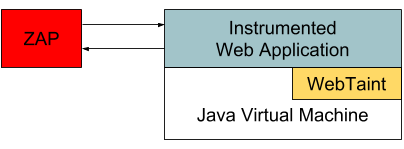
\includegraphics[width=0.8\textwidth]{images/ZAPArchitecture.png}
    \caption{High-level architecture of the ZAP analysing WebTaint enabled web application.}
    \label{fig:ZAP}
\end{figure}

The ZAP accesses the web application over the HTTP protocol and searches for possible vulnerabilities in the applications. An advantage of utilizing a penetration testing tool for evaluation of WebTaint is that vulnerabilities detected by WebTaint are assured to be vulnerabilities if the ZAP detects them as well. However, WebTaint has the possibility of detecting a more extensive set of vulnerabilities since it analyzes applications internally compared to the ZAP which only analyzes externally.

The evaluations of applications are a time-consuming task and therefore only conducted on a smaller set of applications. Each application is a Java-based web application vulnerable to the SQL Injections and Cross-Site Scripting attacks. The web applications are presented in the sections below.



\subsubsection{Stanford SecuriBench Micro}
The Stanford SecuriBench Micro is a set of small test cases designed to evaluate security analyzers. The test suit is deliberately insecure and was created as part of the Griffin Security Project \parencite{griffin} at Stanford University. The application contains 96 test cases and is written in 46407 lines of code. The tests are accessible through input fields on the application. This thesis uses version 1.08 of the application, which is known to contain the vulnerabilities of SQL Injection, Cross-Site Scripting, HTTP Splitting, Path Traversal and more \parencite{securiBenchMicro, microfaq}. 



\subsubsection{InsecureWebApp}
The InsecureWebApp is a deliberately insecure web application developed by OWASP to detect security vulnerabilities and possible harm caused by them. The web application is built for a fictional company called American Service Corporation. Some of the functionalities the application provides are registering, log in, product browsing and placing money into the company account. The vulnerabilities are accessible through the applications input fields and HTTP parameters, and some of them are the Parameter Tampering, Broken Authentication, SQL Injection, HTML Injection, Cross-Site Scripting. The project consists of 2913 lines of code and version 1.0 is used in this thesis \parencite{insecure}. 



\subsubsection{Ticketbook}
The Ticketbook is a deliberately insecure web application developed by Contrast Security to show the power of one of their security tools. The application consists of a set of pages illustrating different security vulnerabilities accessible through input fields and HTTP parameters. Some of these vulnerabilities are the Cross-Site Scripting, Command Injection, SQL Injection, Parameter Tampering, XML External Entity. The application consists of 13849 lines of code and version 0.9.1-SNAPSHOT is used in this thesis \parencite{ticketbook, contrast}.



\subsubsection{SnipSnap}
The SnipSnap is developed to provide the necessary infrastructure to create a collaborative encyclopedia. The web page functionality is similar to the Wikipedia \parencite{wikipedia} where users can sign up and contribute by writing posts. The vulnerabilities in the application are accessible through the different input fields the application utilizes to provide functionalities such as registering and log in. The SnipSnap consists of 566173 lines of code and version 1.0-BETA-1 is used in this thesis \parencite{snipsnap}. The application is not constructed to be deliberately insecure and is intended to be used in production.



\subsubsection{Web Application Policies}
The web applications presented in the previous sections all strive to provide services fulfilling the same policies as described in Section \ref{Integrity} and \ref{Confidentiality}. This emphasizes the fact that all the input fields, HTTP parameters, and other possible user modifiable data are sanitized before being used in the web applications. Possible harmful scenarios of using un-sanitized user input are for example database actions and reflecting information to the user.



\subsection{Micro Benchmarks}
The introduced overhead is measured by the added time and memory overhead. To evaluate these two is the DaCapo Benchmark Suit \parencite{dacapo} used. The DaCapo is a set of applications constructed specifically for benchmarking of Java applications. This thesis uses version DaCapo-9.12-bach which consists of fourteen real-world applications. Table \ref{table:DaCapoTests} contains a description for each application. The summary is taken from the DaCapos website \parencite{dacapoBench}.

\begin{table}[H]
  \centering
  \caption{Descriptions for each application in the DaCapo Benchmark Suit \parencite{dacapoBench}}
    \label{table:DaCapoTests}
    \begin{description}
        \item [Avrora] Simulates a number of programs run on a grid of AVR microcontrollers.
        \item [Batik] Produces a number of Scalable Vector Graphics (SVG) images based on the unit tests in Apache Batik.
        \item [Eclipse] Executes some of the (non-gui) jdt performance tests for the Eclipse IDE.
        \item [Fop] Takes an XSL-FO file, parses it and formats it, generating a PDF file.
        \item [H2] Executes a JDBCbench-like in-memory benchmark, executing a number of transactions against a model of a banking application, replacing the hsqldb benchmark.
        \item [Jython] Interprets a the pybench Python benchmark.
        \item [Luindex] Uses lucene to indexes a set of documents; the works of Shakespeare and the King James Bible.
        \item [Lusearch] Uses lucene to do a text search of keywords over a corpus of data comprising the works of Shakespeare and the King James Bible.
        \item [Pmd] Analyzes a set of Java classes for a range of source code problems.
        \item [Sunflow] Renders a set of images using ray tracing.
        \item [Tomcat] Runs a set of queries against a Tomcat server retrieving and verifying the resulting web pages.
        \item [Tradebeans] Runs the daytrader benchmark via a Jave Beans to a GERONIMO backend with an in-memory h2 as the underlying database.
        \item [Tradesoap] Runs the daytrader benchmark via a SOAP to a GERONIMO backend with in-memory h2 as the underlying database.
        \item [Xalan] Transforms XML documents into HTML.
    \end{description}
\end{table}

The measurement of introduced time and memory is conducted through a C script constructed to execute each application in the DaCapo Benchmark Suit ten times, both with and without WebTaint. Each measurement is executed in an isolated process one at a time to allow accurate memory and time measurements.